\chapter[Experimentos e Resultados]{Experimentos e Resultados}
\label{cap:experimentos}

Neste capítulo são descritos os experimentos conduzidos no desenvolvimento do
RECLin-PT, com foco na classe \texttt{negation\_of}, bem como os resultados obtidos
até o momento, todos no conjunto de desenvolvimento. Os experimentos cruzam as duas
dimensões do desenvolvimento: três \emph{encoders} (BioBERTpt-all, BioBERTpt-clin e
BERTimbau-base) e três estratégias de modelagem (baseline, Pair-Aware linear e
Two-Stage), além da variante exploratória Pair-Aware MLP e dos controles do
protocolo, todos descritos no Capítulo~\ref{cap:prototipo}. Como a Pair-Aware linear é
a arquitetura oficial do RECLin-PT (Seção~\ref{sec:pairaware}), os resultados são
organizados em torno dela: como se compara às demais estratégias e como varia com o
\emph{encoder}. Este capítulo reporta o que foi observado; a interpretação desses
resultados para o RECLin-PT está no Capítulo~\ref{cap:discussao}.

A \autoref{fig:ciclo} situa esses resultados no ciclo de desenvolvimento. A preparação
dos dados, a geração de pares candidatos, o \emph{fine-tuning} das nove combinações de
\emph{encoder} e estratégia e a seleção de épocas e de limiares no DEV estão
concluídos. Permanecem pendentes os experimentos de aprimoramento, a seleção e o
congelamento da configuração final e a avaliação única desse modelo final no conjunto
de teste. A seta de retorno indica que novos \emph{encoders}, hiperparâmetros ou
estratégias voltam à etapa de \emph{fine-tuning} antes de entrar na comparação,
sempre no DEV.

% Ciclo de desenvolvimento do RECLin-PT, com o estado de cada etapa conferido
% nos artefatos (branch resultados-colab, commit ad7c2a2) e no protocolo.
\begin{figure}[htbp]
  \centering
  \caption{Ciclo de desenvolvimento do RECLin-PT e estado atual de cada etapa.}
  \label{fig:ciclo}
  \begin{tikzpicture}[
      font=\sffamily\footnotesize,
      etapa/.style={rounded corners=3pt, minimum height=1.25cm, text width=3.0cm, align=center, inner sep=3pt},
      concluida/.style={etapa, draw=black!80, fill=black!20, line width=0.8pt},
      parcial/.style={etapa, draw=black!80, line width=0.8pt, fill=white, pattern=north east lines, pattern color=black!25},
      pendente/.style={etapa, draw=black!60, dashed, line width=0.8pt, fill=white},
      seta/.style={-{Stealth[length=2.2mm]}, line width=0.8pt},
      estado/.style={font=\sffamily\scriptsize\itshape, text=black!70, below=1.5pt}
    ]
    % linha 1 (da esquerda para a direita)
    \node[concluida] (e1) at (0,0)    {\textbf{1.} Preparação\\ dos dados};
    \node[concluida] (e2) at (3.75,0) {\textbf{2.} Geração de\\ pares candidatos};
    \node[parcial]   (e3) at (7.5,0)  {\textbf{3.} \emph{Fine-tuning}\\ (\emph{encoder} $\times$ estratégia)};
    \node[concluida] (e4) at (11.25,0){\textbf{4.} Seleção de épocas\\ e limiares no DEV};
    % linha 2 (da direita para a esquerda)
    \node[parcial]   (e5) at (11.25,-3.4) {\textbf{5.} Comparação de\\ estratégias e \emph{encoders}};
    \node[pendente]  (e6) at (7.5,-3.4)   {\textbf{6.} Seleção da\\ configuração final};
    \node[pendente]  (e7) at (3.75,-3.4)  {\textbf{7.} Congelamento do\\ modelo final};
    \node[pendente]  (e8) at (0,-3.4)     {\textbf{8.} Avaliação única do\\ modelo final no TEST};
    \draw[seta] (e1) -- (e2);
    \draw[seta] (e2) -- (e3);
    \draw[seta] (e3) -- (e4);
    \draw[seta] (e4.south) -- (e5.north);
    \draw[seta] (e5) -- (e6);
    \draw[seta] (e6) -- (e7);
    \draw[seta] (e7) -- (e8);
    % retorno 5 -> 3
    \draw[seta, dashed] (9.95,-2.775) -- (9.95,-1.7) -- (8.35,-1.7) -- (8.35,-0.625);
    \node[font=\sffamily\scriptsize, anchor=north east] at (9.85,-1.78) {novos \emph{encoders} ou estratégias};
    % estados
    \node[estado] at (e1.south) {concluída};
    \node[estado] at (e2.south) {concluída};
    \node[estado, xshift=-6mm] at (e3.south) {parcial$^{a}$};
    \node[estado, xshift=-8mm] at (e4.south) {concluída$^{b}$};
    \node[estado, xshift=-8mm] at (e5.south) {parcial$^{c}$};
    \node[estado] at (e6.south) {pendente};
    \node[estado] at (e7.south) {pendente};
    \node[estado] at (e8.south) {pendente};
    % legenda
    \begin{scope}[shift={(3.9,-4.95)}, font=\sffamily\scriptsize]
      \node[draw=black!80, fill=black!20, minimum width=5mm, minimum height=3.2mm, rounded corners=1pt] (l1) at (0,0) {};
      \node[right=1mm of l1] (t1) {concluída};
      \node[draw=black!80, fill=white, pattern=north east lines, pattern color=black!25, minimum width=5mm, minimum height=3.2mm, rounded corners=1pt, right=6mm of t1] (l2) {};
      \node[right=1mm of l2] (t2) {parcial};
      \node[draw=black!60, dashed, fill=white, minimum width=5mm, minimum height=3.2mm, rounded corners=1pt, right=6mm of t2] (l3) {};
      \node[right=1mm of l3] {pendente};
    \end{scope}
  \end{tikzpicture}\\[4pt]
  {\footnotesize $^{a}$ Baseline, Pair-Aware linear e Two-Stage foram ajustados com os três \emph{encoders} (BioBERTpt-all, BioBERTpt-clin e BERTimbau-base); a Pair-Aware MLP, só com o BioBERTpt-all; o \emph{fine-tuning} restrito não tem execução. $^{b}$ Para as execuções existentes e verificadas. $^{c}$ Comparações descritivas no DEV; os controles do protocolo existem só com o BioBERTpt-all. Configuração de referência atual: Pair-Aware linear, BioBERTpt-all, semente 42. Pela emenda proposta (E3), novos experimentos voltam à etapa 3 só com treino e DEV, e o TEST avalia apenas o modelo final.}\\[2pt]
  {\footnotesize Fonte: elaborado pelo autor.}
\end{figure}


Todos os números são do conjunto de desenvolvimento (DEV), com semente $42$, sobre os
$19\,064$ pares candidatos das partições congeladas (Seção~\ref{sec:candidatos}). O
DEV é o mesmo conjunto usado nas escolhas de época e de limiar, e nenhuma das
configurações deste trabalho foi avaliada no teste (Seção~\ref{sec:protocolo}). Os
resultados são, portanto, evidências preliminares, e não estimativas finais de
desempenho. Os do Two-Stage e do baseline calibrado, cujo limiar foi escolhido neste
mesmo DEV, são otimistas por construção (Seção~\ref{sec:protocolo}).

\section{Execuções e conferência dos registros}
\label{sec:inventario}

Antes da análise, todas as execuções disponíveis foram inventariadas e conferidas a
partir dos próprios arquivos gravados (Apêndice~\ref{ap:inventario}): $7$ execuções
treinadas de três rótulos (baseline e Pair-Aware linear com os três
\emph{encoders} e a Pair-Aware MLP com o BioBERTpt-all), $6$ estágios do Two-Stage
(dois por \emph{encoder}), $3$ composições do Two-Stage, cada uma com o seu limiar
$\tau$ congelado, e as $2$ execuções derivadas do baseline BioBERTpt-all (baseline
calibrado e filtro léxico). Todas as execuções treinadas estão concluídas, usam a
semente $42$, as mesmas partições (os mesmos \emph{hashes} de treino e de DEV) e a
mesma revisão de pesos por \emph{encoder}. As execuções de três rótulos registram que
o teste não foi avaliado. Os estágios do Two-Stage não têm esse campo, e nenhuma
execução ou composição tem métrica de teste gravada.

As métricas foram recalculadas a partir das predições gravadas e coincidem, valor a
valor, com as registradas por cada execução. Os rótulos de referência das predições
coincidem com os do DEV reconstruído da partição congelada. Cada composição do
Two-Stage foi ligada aos seus dois estágios pelos \emph{hashes} da configuração e do
melhor modelo. Na composição com o BERTimbau-base, os nomes dos estágios registrados
no arquivo do limiar diferem dos nomes das pastas, mas os dois \emph{hashes}
coincidem, o que identifica os mesmos estágios. Os \emph{checkpoints} e os registros
de console das sessões ficam fora do repositório e não foram verificados. Sete
execuções foram interrompidas e retomadas a partir de um \emph{checkpoint} e
registram apenas a sessão final (Apêndice~\ref{ap:historico}).

\section{Treino e seleção de época}
\label{sec:curvas}

Nas sete execuções de três rótulos, a época selecionada foi sempre a terceira, a
última permitida pelo protocolo, e o macro-F1 do DEV ainda subia entre a segunda e a
terceira época em todas elas (na Pair-Aware linear com o BioBERTpt-all, de $0{,}727$
para $0{,}741$). A evolução completa por época, com perdas e duração, está no
Apêndice~\ref{ap:historico}. Em todas, a perda do DEV foi menor na segunda época do
que na terceira, de modo que perda e macro-F1 não apontaram a mesma época. A
coincidência entre a melhor época e o teto é compatível com a possibilidade de que um
orçamento maior de treino altere os números absolutos. Essa possibilidade é comum a
todas as estratégias e não foi explorada. As épocas executadas em uma única sessão
levaram cerca de uma hora na GPU T4. As interrompidas e retomadas registram apenas a
parte final, o que impede usar as durações para comparar o custo das estratégias.

O Two-Stage não segue esse padrão porque seus dois estágios são classificadores
binários treinados separadamente, com critérios de seleção próprios, e o macro-F1 do
\emph{pipeline} completo só é definido após a escolha do limiar~$\tau$
(Seção~\ref{sec:resultados_twostage}).

\section{Visão geral}
\label{sec:resultados}

A Tabela~\ref{tab:dev_sistemas} reúne os doze sistemas com resultado no DEV. Na
classe-alvo, os F1 ficam entre $0{,}800$ e $0{,}832$, faixa que corresponde a poucas
predições: com $150$ pares \texttt{negation\_of} no DEV, os sistemas diferem em no
máximo $14$ verdadeiros positivos e $29$ falsos positivos. Em todos os
\emph{encoders}, a Pair-Aware linear tem F1 de \texttt{negation\_of} maior que o do
baseline (de $0{,}829$, $0{,}826$ e $0{,}818$, contra $0{,}802$, $0{,}814$ e $0{,}800$,
para o BioBERTpt-all, o BioBERTpt-clin e o BERTimbau-base), com \emph{recall} entre
$0{,}940$ e $0{,}960$. O Two-Stage tem os dois maiores F1 de \texttt{negation\_of}, com
os dois BioBERTpt ($0{,}831$ e $0{,}832$), e as três maiores precisões, mas com
\emph{recall} menor. No macro-F1, a Pair-Aware linear com o BioBERTpt-clin
($0{,}746$) só fica abaixo do Two-Stage com o BERTimbau-base ($0{,}751$), e tem o
maior MCC ($0{,}514$). Entre os controles, o filtro léxico e o baseline calibrado
elevam a precisão do baseline ao custo de parte do \emph{recall}: o filtro rebaixou
$24$ das $204$ predições \texttt{negation\_of} do baseline, e o limiar escolhido para
o calibrado foi $t=0{,}90$.

%% GERADO por analise/gerar_tabelas_etapa3.py -- nao edite a mao.
\begin{table}[htbp]
  \centering
  \caption{Resultados no DEV das três estratégias com os três \emph{encoders}, da variante MLP e dos controles: precisão (P), \emph{recall} (R) e F1 de \texttt{negation\_of}, VP/FP/FN, F1 das outras classes, macro-F1 e MCC.}
  \label{tab:dev_sistemas}
  \small\setlength{\tabcolsep}{4pt}
\adjustbox{max width=\textwidth}{%
  \begin{tabular}{llrrrrrrrr}
  \toprule
  Estratégia & \emph{Encoder} & \begin{tabular}[b]{@{}c@{}}P\\neg\end{tabular} & \begin{tabular}[b]{@{}c@{}}R\\neg\end{tabular} & \begin{tabular}[b]{@{}c@{}}F1\\neg\end{tabular} & \begin{tabular}[b]{@{}c@{}}VP/FP/FN\\neg\end{tabular} & \begin{tabular}[b]{@{}c@{}}F1\\assoc\end{tabular} & \begin{tabular}[b]{@{}c@{}}F1\\no\_rel\end{tabular} & Macro-F1 & MCC \\
  \midrule
Pair-Aware linear & BioBERTpt-all & 0{,}742 & 0{,}940 & 0{,}829 & 141/49/9 & 0{,}436 & 0{,}956 & 0{,}741 & 0{,}497 \\
 & BioBERTpt-clin & 0{,}732 & 0{,}947 & 0{,}826 & 142/52/8 & 0{,}454 & 0{,}958 & 0{,}746 & 0{,}514 \\
 & BERTimbau-base & 0{,}713 & 0{,}960 & 0{,}818 & 144/58/6 & 0{,}435 & 0{,}955 & 0{,}736 & 0{,}497 \\
\midrule
Baseline & BioBERTpt-all & 0{,}696 & 0{,}947 & 0{,}802 & 142/62/8 & 0{,}408 & 0{,}946 & 0{,}719 & 0{,}480 \\
 & BioBERTpt-clin & 0{,}722 & 0{,}933 & 0{,}814 & 140/54/10 & 0{,}426 & 0{,}952 & 0{,}731 & 0{,}489 \\
 & BERTimbau-base & 0{,}708 & 0{,}920 & 0{,}800 & 138/57/12 & 0{,}417 & 0{,}951 & 0{,}723 & 0{,}480 \\
\midrule
Two-Stage & BioBERTpt-all ($\tau=0{,}95$) & 0{,}798 & 0{,}867 & 0{,}831 & 130/33/20 & 0{,}366 & 0{,}978 & 0{,}725 & 0{,}462 \\
 & BioBERTpt-clin ($\tau=0{,}95$) & 0{,}768 & 0{,}907 & 0{,}832 & 136/41/14 & 0{,}380 & 0{,}977 & 0{,}730 & 0{,}464 \\
 & BERTimbau-base ($\tau=0{,}85$) & 0{,}753 & 0{,}913 & 0{,}825 & 137/45/13 & 0{,}461 & 0{,}968 & 0{,}751 & 0{,}505 \\
\midrule
Pair-Aware MLP & BioBERTpt-all & 0{,}715 & 0{,}953 & 0{,}817 & 143/57/7 & 0{,}438 & 0{,}956 & 0{,}737 & 0{,}498 \\
\midrule
Baseline calibrado & BioBERTpt-all ($t=0{,}90$) & 0{,}723 & 0{,}920 & 0{,}809 & 138/53/12 & 0{,}407 & 0{,}946 & 0{,}721 & 0{,}479 \\
\midrule
Filtro léxico & BioBERTpt-all & 0{,}750 & 0{,}900 & 0{,}818 & 135/45/15 & 0{,}408 & 0{,}946 & 0{,}724 & 0{,}477 \\
  \bottomrule
  \end{tabular}}\\[2pt]
  {\footnotesize DEV, $n=19\,064$ pares candidatos (150 \texttt{negation\_of}, 763 \texttt{associated\_with}), semente 42. Não são resultados de teste. A época de cada modelo, $\tau$ (Two-Stage) e $t$ (baseline calibrado) foram escolhidos neste mesmo DEV. O protocolo pré-registrado fixa o BioBERTpt-all; as execuções com o BioBERTpt-clin e o BERTimbau-base são variantes de \emph{encoder} fora do pré-registro, e a Pair-Aware MLP é exploratória.}\\[4pt]
  {\footnotesize Fonte: elaborado pelo autor.}
\end{table}


As outras duas classes completam o quadro (Tabela~\ref{tab:dev_classes}). Em
\texttt{associated\_with}, todas as estratégias treinadas de três rótulos têm \emph{recall}
entre $0{,}760$ e $0{,}826$ e precisão entre $0{,}271$ e $0{,}319$. A Pair-Aware linear
tem precisão maior que a do baseline nos três \emph{encoders}. O Two-Stage com os dois
BioBERTpt inverte esse perfil: precisão de cerca de $0{,}5$ e \emph{recall} de cerca
de $0{,}3$. Com o BERTimbau-base, cujo limiar é menor, o Two-Stage fica entre os dois
perfis e tem o maior F1 da classe ($0{,}461$). A AP de \texttt{associated\_with}, que
não depende de limiar, vai de $0{,}396$ a $0{,}446$ nas estratégias de três rótulos e é
maior na Pair-Aware linear do que no baseline nos três \emph{encoders}.

%% GERADO por analise/gerar_tabelas_etapa3.py -- nao edite a mao.
\begin{table}[htbp]
  \centering
  \caption{\texttt{associated\_with} e \texttt{no\_relation} no DEV: precisão, \emph{recall}, F1, VP/FP/FN e AP de \texttt{associated\_with}.}
  \label{tab:dev_classes}
  \small\setlength{\tabcolsep}{4pt}
\adjustbox{max width=\textwidth}{%
  \begin{tabular}{llrrrrrrrr}
  \toprule
  & & \multicolumn{5}{c}{\texttt{associated\_with}} & \multicolumn{3}{c}{\texttt{no\_relation}} \\
  \cmidrule(lr){3-7}\cmidrule(lr){8-10}
  Estratégia & \emph{Encoder} & P & R & F1 & VP/FP/FN & AP & P & R & F1 \\
  \midrule
Pair-Aware linear & BioBERTpt-all & 0{,}305 & 0{,}764 & 0{,}436 & 583/1326/180 & 0{,}445 & 0{,}989 & 0{,}925 & 0{,}956 \\
 & BioBERTpt-clin & 0{,}319 & 0{,}785 & 0{,}454 & 599/1276/164 & 0{,}446 & 0{,}990 & 0{,}927 & 0{,}958 \\
 & BERTimbau-base & 0{,}304 & 0{,}765 & 0{,}435 & 584/1340/179 & 0{,}413 & 0{,}990 & 0{,}923 & 0{,}955 \\
\midrule
Baseline & BioBERTpt-all & 0{,}271 & 0{,}826 & 0{,}408 & 630/1696/133 & 0{,}425 & 0{,}992 & 0{,}904 & 0{,}946 \\
 & BioBERTpt-clin & 0{,}292 & 0{,}785 & 0{,}426 & 599/1453/164 & 0{,}416 & 0{,}990 & 0{,}917 & 0{,}952 \\
 & BERTimbau-base & 0{,}285 & 0{,}782 & 0{,}417 & 597/1501/166 & 0{,}396 & 0{,}990 & 0{,}915 & 0{,}951 \\
\midrule
Two-Stage & BioBERTpt-all ($\tau=0{,}95$) & 0{,}508 & 0{,}286 & 0{,}366 & 218/211/545 & -- & 0{,}970 & 0{,}987 & 0{,}978 \\
 & BioBERTpt-clin ($\tau=0{,}95$) & 0{,}481 & 0{,}315 & 0{,}380 & 240/259/523 & -- & 0{,}971 & 0{,}984 & 0{,}977 \\
 & BERTimbau-base ($\tau=0{,}85$) & 0{,}364 & 0{,}626 & 0{,}461 & 478/834/285 & -- & 0{,}984 & 0{,}952 & 0{,}968 \\
\midrule
Pair-Aware MLP & BioBERTpt-all & 0{,}308 & 0{,}760 & 0{,}438 & 580/1305/183 & 0{,}436 & 0{,}989 & 0{,}925 & 0{,}956 \\
\midrule
Baseline calibrado & BioBERTpt-all ($t=0{,}90$) & 0{,}270 & 0{,}826 & 0{,}407 & 630/1700/133 & 0{,}425 & 0{,}992 & 0{,}904 & 0{,}946 \\
\midrule
Filtro léxico & BioBERTpt-all & 0{,}271 & 0{,}826 & 0{,}408 & 630/1696/133 & -- & 0{,}992 & 0{,}905 & 0{,}946 \\
  \bottomrule
  \end{tabular}}\\[2pt]
  {\footnotesize AP: precisão média de \texttt{associated\_with} calculada das probabilidades gravadas, sem limiar; não se aplica ao Two-Stage (as probabilidades do estágio 2 não são gravadas) nem ao filtro léxico (pós-processamento sem probabilidades próprias). O baseline calibrado usa as probabilidades do baseline, por isso a mesma AP.}\\[4pt]
  {\footnotesize Fonte: elaborado pelo autor.}
\end{table}


A \autoref{fig:confusao} mostra para onde vão os erros, com o BioBERTpt-all. No
baseline e na Pair-Aware linear, a classe \texttt{negation\_of} é quase toda
recuperada, e o erro dominante é a confusão de \texttt{no\_relation} com
\texttt{associated\_with} ($1\,693$ e $1\,323$ pares). No Two-Stage, essa confusão
quase desaparece ($208$ pares), mas o erro se desloca para o sentido inverso: $541$
das $763$ relações \texttt{associated\_with} são classificadas como
\texttt{no\_relation}, e $17$ das $150$ \texttt{negation\_of} também.

\begin{figure}[htbp]
  \centering
  \caption{Matrizes de confusão no DEV (normalizadas por linha, contagens entre parênteses): baseline, Pair-Aware linear e Two-Stage, BioBERTpt-all, seed 42.}
  \label{fig:confusao}
  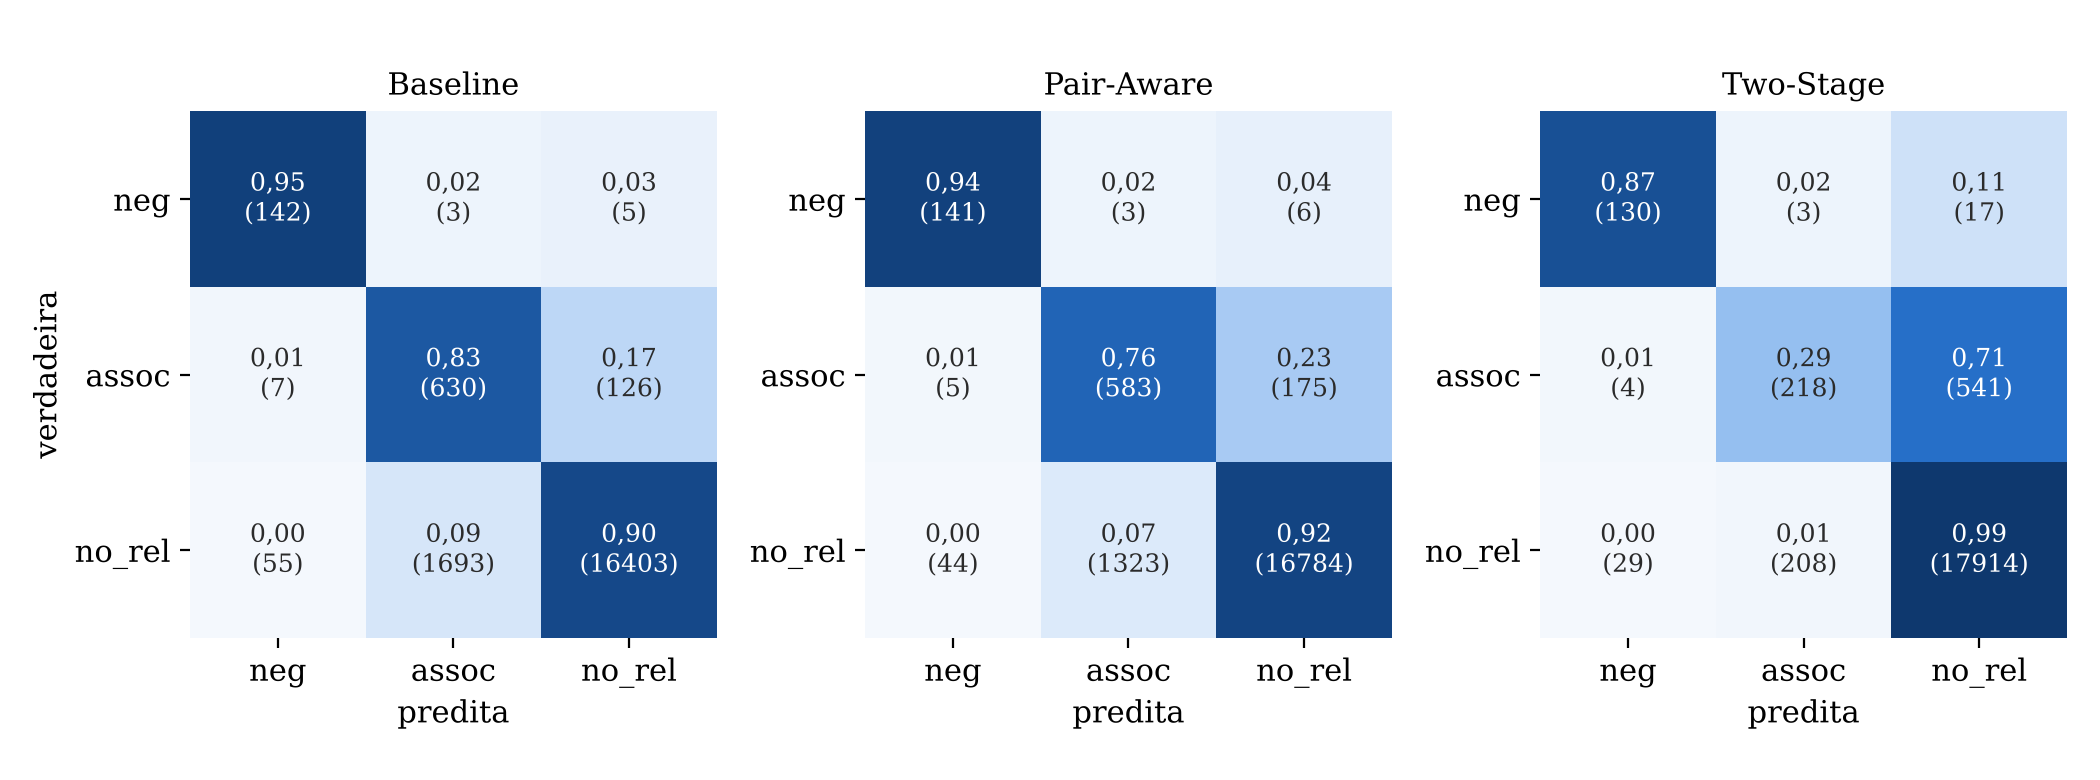
\includegraphics[width=\textwidth]{resultados/matrizes_confusao_dev.png}\\[4pt]
  {\footnotesize Fonte: elaborado pelo autor.}
\end{figure}

\section{A Pair-Aware linear frente às demais estratégias}
\label{sec:resultados_comparacoes}

A Tabela~\ref{tab:dev_comparacoes_pa} aplica ao DEV, de forma descritiva, os testes
pareados da Seção~\ref{sec:avaliacao}, com dois níveis de reamostragem: por candidato,
como prevê o protocolo, e por documento, que reamostra inteiros os $98$ documentos do
DEV que têm pares candidatos e leva em conta que pares de um mesmo documento não são
independentes. Os resultados estão organizados em um bloco por métrica, cada um com
os intervalos dos dois níveis. Os intervalos por documento são, em geral, mais
largos.

%% GERADO por analise/gerar_tabelas_etapa3.py -- nao edite a mao.
\begingroup\small\renewcommand{\arraystretch}{1.2}\setlength{\tabcolsep}{4pt}
\setlength{\LTleft}{0pt}\setlength{\LTright}{0pt}\setlength{\LTcapwidth}{\textwidth}
\Needspace*{0.3\textheight}
\begin{longtable}{@{\extracolsep{\fill}}llrcc}
\caption{Comparações pareadas descritivas da Pair-Aware linear, no DEV, por métrica: diferenças e intervalos de confiança de F1 de \texttt{negation\_of}, de F1 de \texttt{associated\_with} e de macro-F1.}\label{tab:dev_comparacoes_pa} \\
\toprule
B (A = Pair-Aware linear) & \emph{Encoder} & $\Delta$ & IC95\% (candidato) & IC95\% (documento) \\
\midrule
\endfirsthead
\multicolumn{5}{l}{\footnotesize Tabela~\thetable{} -- continuação} \\
\toprule
B (A = Pair-Aware linear) & \emph{Encoder} & $\Delta$ & IC95\% (candidato) & IC95\% (documento) \\
\midrule
\endhead
\midrule
\multicolumn{5}{r}{\footnotesize continua} \\
\endfoot
\bottomrule
\endlastfoot
\multicolumn{5}{l}{\textit{Métrica:} F1 de \texttt{negation\_of}} \\*
Baseline & BioBERTpt-all & $+0{,}0272$ & $[+0{,}005;\,+0{,}051]$$^{\ast}$ & $[+0{,}001;\,+0{,}056]$$^{\ast}$ \\
Baseline & BioBERTpt-clin & $+0{,}0116$ & $[-0{,}009;\,+0{,}034]$ & $[-0{,}008;\,+0{,}032]$ \\
Baseline & BERTimbau-base & $+0{,}0182$ & $[-0{,}009;\,+0{,}046]$ & $[-0{,}011;\,+0{,}045]$ \\
Two-Stage & BioBERTpt-all & $-0{,}0013$ & $[-0{,}035;\,+0{,}033]$ & $[-0{,}033;\,+0{,}030]$ \\
Two-Stage & BioBERTpt-clin & $-0{,}0062$ & $[-0{,}037;\,+0{,}026]$ & $[-0{,}039;\,+0{,}026]$ \\
Two-Stage & BERTimbau-base & $-0{,}0071$ & $[-0{,}036;\,+0{,}022]$ & $[-0{,}048;\,+0{,}029]$ \\
Pair-Aware MLP & BioBERTpt-all & $+0{,}0123$ & $[-0{,}011;\,+0{,}036]$ & $[-0{,}011;\,+0{,}037]$ \\
Baseline calibrado & BioBERTpt-all & $+0{,}0200$ & $[0{,}000;\,+0{,}042]$ & $[-0{,}002;\,+0{,}043]$ \\
Filtro léxico & BioBERTpt-all & $+0{,}0112$ & $[-0{,}013;\,+0{,}036]$ & $[-0{,}017;\,+0{,}039]$ \\
\midrule
\multicolumn{5}{l}{\textit{Métrica:} F1 de \texttt{associated\_with}} \\*
Baseline & BioBERTpt-all & $+0{,}0285$ & $[+0{,}015;\,+0{,}042]$$^{\ast}$ & $[+0{,}009;\,+0{,}046]$$^{\ast}$ \\
Baseline & BioBERTpt-clin & $+0{,}0286$ & $[+0{,}016;\,+0{,}042]$$^{\ast}$ & $[+0{,}014;\,+0{,}042]$$^{\ast}$ \\
Baseline & BERTimbau-base & $+0{,}0173$ & $[+0{,}005;\,+0{,}029]$$^{\ast}$ & $[+0{,}005;\,+0{,}030]$$^{\ast}$ \\
Two-Stage & BioBERTpt-all & $+0{,}0706$ & $[+0{,}035;\,+0{,}106]$$^{\ast}$ & $[+0{,}013;\,+0{,}126]$$^{\ast}$ \\
Two-Stage & BioBERTpt-clin & $+0{,}0738$ & $[+0{,}039;\,+0{,}108]$$^{\ast}$ & $[+0{,}014;\,+0{,}135]$$^{\ast}$ \\
Two-Stage & BERTimbau-base & $-0{,}0260$ & $[-0{,}043;\,-0{,}008]$$^{\ast}$ & $[-0{,}051;\,+0{,}001]$ \\
Pair-Aware MLP & BioBERTpt-all & $-0{,}0017$ & $[-0{,}013;\,+0{,}010]$ & $[-0{,}015;\,+0{,}011]$ \\
Baseline calibrado & BioBERTpt-all & $+0{,}0290$ & $[+0{,}015;\,+0{,}042]$$^{\ast}$ & $[+0{,}009;\,+0{,}047]$$^{\ast}$ \\
Filtro léxico & BioBERTpt-all & $+0{,}0285$ & $[+0{,}015;\,+0{,}042]$$^{\ast}$ & $[+0{,}009;\,+0{,}046]$$^{\ast}$ \\
\midrule
\multicolumn{5}{l}{\textit{Métrica:} Macro-F1} \\*
Baseline & BioBERTpt-all & $+0{,}0219$ & $[+0{,}013;\,+0{,}031]$$^{\ast}$ & $[+0{,}010;\,+0{,}034]$$^{\ast}$ \\
Baseline & BioBERTpt-clin & $+0{,}0151$ & $[+0{,}006;\,+0{,}024]$$^{\ast}$ & $[+0{,}007;\,+0{,}023]$$^{\ast}$ \\
Baseline & BERTimbau-base & $+0{,}0134$ & $[+0{,}003;\,+0{,}024]$$^{\ast}$ & $[+0{,}004;\,+0{,}023]$$^{\ast}$ \\
Two-Stage & BioBERTpt-all & $+0{,}0157$ & $[-0{,}001;\,+0{,}032]$ & $[-0{,}008;\,+0{,}038]$ \\
Two-Stage & BioBERTpt-clin & $+0{,}0159$ & $[+0{,}0004;\,+0{,}032]$$^{\ast}$ & $[-0{,}008;\,+0{,}040]$ \\
Two-Stage & BERTimbau-base & $-0{,}0151$ & $[-0{,}027;\,-0{,}003]$$^{\ast}$ & $[-0{,}033;\,+0{,}001]$ \\
Pair-Aware MLP & BioBERTpt-all & $+0{,}0034$ & $[-0{,}005;\,+0{,}012]$ & $[-0{,}005;\,+0{,}013]$ \\
Baseline calibrado & BioBERTpt-all & $+0{,}0196$ & $[+0{,}011;\,+0{,}029]$$^{\ast}$ & $[+0{,}009;\,+0{,}030]$$^{\ast}$ \\
Filtro léxico & BioBERTpt-all & $+0{,}0165$ & $[+0{,}007;\,+0{,}026]$$^{\ast}$ & $[+0{,}006;\,+0{,}027]$$^{\ast}$ \\
\end{longtable}
\vspace{-\baselineskip}
\nopagebreak\noindent\begin{minipage}{\linewidth}
{\footnotesize Descritivas, no DEV: as épocas, $\tau$ e $t$ foram escolhidos neste mesmo conjunto; não substituem as comparações pré-registradas no teste. A é a Pair-Aware linear; A e B usam o mesmo \emph{encoder}. $\Delta$: diferença observada A $-$ B no DEV completo. IC95\% (candidato): \emph{bootstrap} pareado que reamostra com reposição os 19\,064 pares candidatos, o do protocolo (10.000 reamostras, semente 42). IC95\% (documento): \emph{bootstrap} pareado que reamostra com reposição os 98 documentos do DEV que têm pares candidatos, cada um com todos os seus pares (10.000 reamostras, semente 42). As três métricas são calculadas sobre as mesmas reamostras de cada nível. Intervalos: percentis 2,5 e 97,5 das diferenças reamostradas. $^{\ast}$: intervalo que exclui o zero. Limites que arredondariam a zero com três casas aparecem com mais casas. O teste de McNemar dessas comparações está no Quadro~\ref{quad:mcnemar}.\par}\vspace{4pt}
{\footnotesize Fonte: elaborado pelo autor.}
\end{minipage}\par
\endgroup


Contra o baseline do mesmo \emph{encoder}, a Pair-Aware linear tem diferença
detectada no macro-F1 e no F1 de \texttt{associated\_with} nos três
\emph{encoders}, nos dois níveis de reamostragem. No F1 de \texttt{negation\_of},
a diferença só é detectada com o BioBERTpt-all ($+0{,}027$, com IC95\% de
$[+0{,}005;\,+0{,}051]$ por candidato e de $[+0{,}001;\,+0{,}056]$ por documento). Com
o BioBERTpt-clin ($+0{,}012$) e o BERTimbau-base ($+0{,}018$), os intervalos contêm o
zero.

Contra o Two-Stage do mesmo \emph{encoder}, nenhuma diferença no F1 de
\texttt{negation\_of} é detectada (de $-0{,}001$ a $-0{,}007$). As diferenças nas
outras classes dependem do \emph{encoder}, porque dependem do limiar do Two-Stage:
com os dois BioBERTpt ($\tau=0{,}95$), a Pair-Aware linear tem F1 de
\texttt{associated\_with} maior ($+0{,}071$ e $+0{,}074$, detectado nos dois níveis), e
a diferença no macro-F1 ($+0{,}016$) só é detectada por candidato com o
BioBERTpt-clin; com o BERTimbau-base ($\tau=0{,}85$), o Two-Stage tem F1 de
\texttt{associated\_with} e macro-F1 maiores, com diferença detectada por candidato,
mas não por documento.

Com o BioBERTpt-all, a Pair-Aware linear também foi comparada à variante MLP e aos
controles. Com a MLP, nenhuma diferença é detectada. Contra o baseline calibrado, a
diferença no F1 de \texttt{negation\_of} é de $+0{,}020$, com limite inferior do
IC95\% igual a zero por candidato e abaixo de zero por documento, e contra o filtro
léxico, de $+0{,}011$, também não detectada. No macro-F1 e em
\texttt{associated\_with}, a diferença é detectada contra os dois controles, que
praticamente não alteram essas classes. O McNemar, apresentado à parte no
Quadro~\ref{quad:mcnemar}, rejeita a igualdade em quase todas as comparações, mas
responde a outra pergunta: ele incide sobre o acerto global, dominado pela classe
\texttt{no\_relation}, e não é específico de nenhuma classe. Entre as comparações da
Pair-Aware linear, a exceção é a comparação com a variante MLP ($b/c$ de $249/261$).

%% GERADO por analise/gerar_tabelas_etapa3.py -- nao edite a mao.
\begin{quadro}[htbp]
  \centering
  \caption{Teste de McNemar das comparações pareadas entre estratégias, no DEV.}
  \label{quad:mcnemar}
  \small
  \begin{tabular}{llrrr}
  \toprule
  Comparação (A $-$ B) & \emph{Encoder} & $b$ & $c$ & $p$ \\
  \midrule
  \multicolumn{5}{l}{\textit{Pair-Aware linear frente às demais estratégias (Tabela~\ref{tab:dev_comparacoes_pa})}} \\
  Pair-Aware linear $-$ Baseline & BioBERTpt-all & 588 & 255 & $<0{,}0001$ \\
  Pair-Aware linear $-$ Baseline & BioBERTpt-clin & 432 & 254 & $<0{,}0001$ \\
  Pair-Aware linear $-$ Baseline & BERTimbau-base & 423 & 270 & $<0{,}0001$ \\
  Pair-Aware linear $-$ Two-Stage & BioBERTpt-all & 383 & 1\,137 & $<0{,}0001$ \\
  Pair-Aware linear $-$ Two-Stage & BioBERTpt-clin & 376 & 1\,039 & $<0{,}0001$ \\
  Pair-Aware linear $-$ Two-Stage & BERTimbau-base & 183 & 589 & $<0{,}0001$ \\
  Pair-Aware linear $-$ Pair-Aware MLP & BioBERTpt-all & 249 & 261 & $0{,}6262$ \\
  Pair-Aware linear $-$ Baseline calibrado & BioBERTpt-all & 587 & 258 & $<0{,}0001$ \\
  Pair-Aware linear $-$ Filtro léxico & BioBERTpt-all & 589 & 264 & $<0{,}0001$ \\
  \midrule
  \multicolumn{5}{l}{\textit{Two-Stage e baseline calibrado (Tabela~\ref{tab:dev_comparacoes_ts})}} \\
  Two-Stage $-$ Baseline & BioBERTpt-all & 1\,517 & 430 & $<0{,}0001$ \\
  Two-Stage $-$ Baseline & BioBERTpt-clin & 1\,212 & 371 & $<0{,}0001$ \\
  Two-Stage $-$ Baseline & BERTimbau-base & 738 & 179 & $<0{,}0001$ \\
  Two-Stage $-$ Baseline calibrado & BioBERTpt-all & 1\,512 & 429 & $<0{,}0001$ \\
  Baseline calibrado $-$ Baseline & BioBERTpt-all & 8 & 4 & $0{,}3877$ \\
  \bottomrule
  \end{tabular}\\[2pt]
  \parbox{\textwidth}{\footnotesize Teste de McNemar exato sobre o acerto global de cada par candidato do DEV, dominado pela classe \texttt{no\_relation}; não é específico de nenhuma classe. $b$: pares em que só A acerta; $c$: pares em que só B acerta. $p$: valor-$p$ bilateral do teste binomial exato, $b \sim \mathrm{Binomial}(b+c,\,0{,}5)$. Descritivo, no DEV.}\\[4pt]
  {\footnotesize Fonte: elaborado pelo autor.}
\end{quadro}


\section{O efeito do \emph{encoder}}
\label{sec:resultados_encoders}

A Tabela~\ref{tab:dev_comparacoes_encoders} compara os três \emph{encoders} dentro de
cada estratégia, com a mesma configuração e apenas o \emph{checkpoint} de pré-treino
trocado. No F1 de \texttt{negation\_of}, nenhuma das nove comparações tem diferença
detectada. As diferenças vão de $-0{,}011$ a $+0{,}014$. Na Pair-Aware linear, o
BioBERTpt-all tem o maior F1 da classe-alvo ($0{,}829$), o BioBERTpt-clin, o maior
macro-F1 ($0{,}746$), e o BERTimbau-base, o maior \emph{recall} ($0{,}960$) e a menor
precisão ($0{,}713$).

%% GERADO por analise/gerar_tabelas_etapa3.py -- nao edite a mao.
\begingroup\small\renewcommand{\arraystretch}{1.2}\setlength{\tabcolsep}{4pt}
\setlength{\LTleft}{0pt}\setlength{\LTright}{0pt}\setlength{\LTcapwidth}{\textwidth}
\Needspace*{0.3\textheight}
\begin{longtable}{@{\extracolsep{\fill}}lrcc}
\caption{Comparação entre \emph{encoders} dentro de cada estratégia, no DEV, por métrica (mesma configuração; só o \emph{checkpoint} de pré-treino muda).}\label{tab:dev_comparacoes_encoders} \\
\toprule
Estratégia e comparação (A $-$ B) & $\Delta$ & IC95\% (candidato) & IC95\% (documento) \\
\midrule
\endfirsthead
\multicolumn{4}{l}{\footnotesize Tabela~\thetable{} -- continuação} \\
\toprule
Estratégia e comparação (A $-$ B) & $\Delta$ & IC95\% (candidato) & IC95\% (documento) \\
\midrule
\endhead
\midrule
\multicolumn{4}{r}{\footnotesize continua} \\
\endfoot
\bottomrule
\endlastfoot
\multicolumn{4}{l}{\textit{Métrica:} F1 de \texttt{negation\_of}} \\*
\addlinespace[2pt]\multicolumn{4}{l}{\quad\textit{Pair-Aware linear}} \\*
\quad BioBERTpt-clin $-$ BioBERTpt-all & $-0{,}0038$ & $[-0{,}026;\,+0{,}018]$ & $[-0{,}023;\,+0{,}016]$ \\
\quad BERTimbau-base $-$ BioBERTpt-all & $-0{,}0112$ & $[-0{,}036;\,+0{,}013]$ & $[-0{,}038;\,+0{,}014]$ \\
\quad BioBERTpt-clin $-$ BERTimbau-base & $+0{,}0074$ & $[-0{,}013;\,+0{,}029]$ & $[-0{,}014;\,+0{,}029]$ \\
\addlinespace[2pt]\multicolumn{4}{l}{\quad\textit{Baseline}} \\*
\quad BioBERTpt-clin $-$ BioBERTpt-all & $+0{,}0117$ & $[-0{,}013;\,+0{,}036]$ & $[-0{,}009;\,+0{,}035]$ \\
\quad BERTimbau-base $-$ BioBERTpt-all & $-0{,}0023$ & $[-0{,}029;\,+0{,}025]$ & $[-0{,}029;\,+0{,}028]$ \\
\quad BioBERTpt-clin $-$ BERTimbau-base & $+0{,}0140$ & $[-0{,}009;\,+0{,}038]$ & $[-0{,}010;\,+0{,}036]$ \\
\addlinespace[2pt]\multicolumn{4}{l}{\quad\textit{Two-Stage}} \\*
\quad BioBERTpt-clin $-$ BioBERTpt-all & $+0{,}0011$ & $[-0{,}029;\,+0{,}031]$ & $[-0{,}027;\,+0{,}031]$ \\
\quad BERTimbau-base $-$ BioBERTpt-all & $-0{,}0054$ & $[-0{,}037;\,+0{,}026]$ & $[-0{,}036;\,+0{,}026]$ \\
\quad BioBERTpt-clin $-$ BERTimbau-base & $+0{,}0065$ & $[-0{,}026;\,+0{,}039]$ & $[-0{,}027;\,+0{,}040]$ \\
\midrule
\multicolumn{4}{l}{\textit{Métrica:} F1 de \texttt{associated\_with}} \\*
\addlinespace[2pt]\multicolumn{4}{l}{\quad\textit{Pair-Aware linear}} \\*
\quad BioBERTpt-clin $-$ BioBERTpt-all & $+0{,}0178$ & $[+0{,}006;\,+0{,}030]$$^{\ast}$ & $[+0{,}003;\,+0{,}034]$$^{\ast}$ \\
\quad BERTimbau-base $-$ BioBERTpt-all & $-0{,}0017$ & $[-0{,}015;\,+0{,}011]$ & $[-0{,}013;\,+0{,}011]$ \\
\quad BioBERTpt-clin $-$ BERTimbau-base & $+0{,}0194$ & $[+0{,}006;\,+0{,}033]$$^{\ast}$ & $[+0{,}002;\,+0{,}038]$$^{\ast}$ \\
\addlinespace[2pt]\multicolumn{4}{l}{\quad\textit{Baseline}} \\*
\quad BioBERTpt-clin $-$ BioBERTpt-all & $+0{,}0177$ & $[+0{,}005;\,+0{,}030]$$^{\ast}$ & $[+0{,}004;\,+0{,}032]$$^{\ast}$ \\
\quad BERTimbau-base $-$ BioBERTpt-all & $+0{,}0094$ & $[-0{,}003;\,+0{,}022]$ & $[-0{,}008;\,+0{,}025]$ \\
\quad BioBERTpt-clin $-$ BERTimbau-base & $+0{,}0082$ & $[-0{,}005;\,+0{,}021]$ & $[-0{,}009;\,+0{,}025]$ \\
\addlinespace[2pt]\multicolumn{4}{l}{\quad\textit{Two-Stage}} \\*
\quad BioBERTpt-clin $-$ BioBERTpt-all & $+0{,}0146$ & $[-0{,}013;\,+0{,}042]$ & $[-0{,}015;\,+0{,}047]$ \\
\quad BERTimbau-base $-$ BioBERTpt-all & $+0{,}0950$ & $[+0{,}061;\,+0{,}129]$$^{\ast}$ & $[+0{,}052;\,+0{,}138]$$^{\ast}$ \\
\quad BioBERTpt-clin $-$ BERTimbau-base & $-0{,}0804$ & $[-0{,}112;\,-0{,}049]$$^{\ast}$ & $[-0{,}123;\,-0{,}037]$$^{\ast}$ \\
\midrule
\multicolumn{4}{l}{\textit{Métrica:} Macro-F1} \\*
\addlinespace[2pt]\multicolumn{4}{l}{\quad\textit{Pair-Aware linear}} \\*
\quad BioBERTpt-clin $-$ BioBERTpt-all & $+0{,}0052$ & $[-0{,}003;\,+0{,}014]$ & $[-0{,}004;\,+0{,}014]$ \\
\quad BERTimbau-base $-$ BioBERTpt-all & $-0{,}0045$ & $[-0{,}014;\,+0{,}005]$ & $[-0{,}015;\,+0{,}006]$ \\
\quad BioBERTpt-clin $-$ BERTimbau-base & $+0{,}0097$ & $[+0{,}001;\,+0{,}019]$$^{\ast}$ & $[-0{,}001;\,+0{,}020]$ \\
\addlinespace[2pt]\multicolumn{4}{l}{\quad\textit{Baseline}} \\*
\quad BioBERTpt-clin $-$ BioBERTpt-all & $+0{,}0120$ & $[+0{,}003;\,+0{,}021]$$^{\ast}$ & $[+0{,}003;\,+0{,}022]$$^{\ast}$ \\
\quad BERTimbau-base $-$ BioBERTpt-all & $+0{,}0041$ & $[-0{,}006;\,+0{,}014]$ & $[-0{,}006;\,+0{,}015]$ \\
\quad BioBERTpt-clin $-$ BERTimbau-base & $+0{,}0079$ & $[-0{,}001;\,+0{,}017]$ & $[-0{,}001;\,+0{,}017]$ \\
\addlinespace[2pt]\multicolumn{4}{l}{\quad\textit{Two-Stage}} \\*
\quad BioBERTpt-clin $-$ BioBERTpt-all & $+0{,}0049$ & $[-0{,}009;\,+0{,}019]$ & $[-0{,}008;\,+0{,}020]$ \\
\quad BERTimbau-base $-$ BioBERTpt-all & $+0{,}0263$ & $[+0{,}011;\,+0{,}042]$$^{\ast}$ & $[+0{,}007;\,+0{,}046]$$^{\ast}$ \\
\quad BioBERTpt-clin $-$ BERTimbau-base & $-0{,}0213$ & $[-0{,}037;\,-0{,}006]$$^{\ast}$ & $[-0{,}040;\,-0{,}003]$$^{\ast}$ \\
\end{longtable}
\vspace{-\baselineskip}
\nopagebreak\noindent\begin{minipage}{\linewidth}
{\footnotesize Descritivas, no DEV: as épocas, $\tau$ e $t$ foram escolhidos neste mesmo conjunto; não substituem as comparações pré-registradas no teste. A e B usam a mesma estratégia e a mesma configuração; só o \emph{checkpoint} de pré-treino muda. $\Delta$: diferença observada A $-$ B no DEV completo. IC95\% (candidato): \emph{bootstrap} pareado que reamostra com reposição os 19\,064 pares candidatos, o do protocolo (10.000 reamostras, semente 42). IC95\% (documento): \emph{bootstrap} pareado que reamostra com reposição os 98 documentos do DEV que têm pares candidatos, cada um com todos os seus pares (10.000 reamostras, semente 42). As três métricas são calculadas sobre as mesmas reamostras de cada nível. Intervalos: percentis 2,5 e 97,5 das diferenças reamostradas. $^{\ast}$: intervalo que exclui o zero. Limites que arredondariam a zero com três casas aparecem com mais casas.\par}\vspace{4pt}
{\footnotesize Fonte: elaborado pelo autor.}
\end{minipage}\par
\endgroup


As diferenças detectadas aparecem nas outras classes. O BioBERTpt-clin tem F1 de
\texttt{associated\_with} maior que o do BioBERTpt-all na Pair-Aware linear e no
baseline, e maior que o do BERTimbau-base na Pair-Aware linear, nos dois níveis de
reamostragem. No baseline, ele também tem macro-F1 maior que o do BioBERTpt-all. No
Two-Stage, o BERTimbau-base tem F1 de \texttt{associated\_with} e macro-F1 maiores
que os dos dois BioBERTpt, mas essas diferenças acompanham a diferença de limiar
($\tau=0{,}85$ contra $0{,}95$) e não isolam o \emph{encoder}. O BERTimbau-base tem
cerca de 61\% dos parâmetros dos dois BioBERTpt.

\section{A classe \texttt{associated\_with}}
\label{sec:resultados_assoc}

A precisão de \texttt{associated\_with} é a mais baixa das três classes em todos os
sistemas. A Tabela~\ref{tab:dev_assoc_fp} decompõe os falsos positivos dessa classe.
Em todas as estratégias e \emph{encoders}, entre $25\%$ e $31\%$ deles são pares cuja
direção inversa está anotada como \texttt{associated\_with}: o modelo reconhece a
associação entre as duas entidades, mas não a direção anotada. Os demais são, quase
todos, pares sem relação anotada em nenhuma direção. No máximo $1{,}4\%$ são pares
\texttt{negation\_of}. No DEV, só $4$ das $763$ relações \texttt{associated\_with}
candidatas têm o par inverso também anotado, de modo que a direção é, na prática,
sempre uma escolha exclusiva. A precisão também cai com a distância entre os
argumentos: nas estratégias de três rótulos, fica entre $0{,}35$ e $0{,}39$ quando os
argumentos estão a até um caractere e entre $0{,}14$ e $0{,}17$ na faixa de $11$ a $25$
caracteres.

%% GERADO por analise/gerar_tabelas_etapa3.py -- nao edite a mao.
\begin{table}[htbp]
  \centering
  \caption{Falsos positivos de \texttt{associated\_with} no DEV: origem e precisão por faixa de distância entre os argumentos.}
  \label{tab:dev_assoc_fp}
  \small\setlength{\tabcolsep}{4pt}
\adjustbox{max width=\textwidth}{%
  \begin{tabular}{llrrrrrrrr}
  \toprule
  & & & \multicolumn{3}{c}{Origem dos FP} & \multicolumn{4}{c}{Precisão por distância} \\
  \cmidrule(lr){4-6}\cmidrule(lr){7-10}
  Estratégia & \emph{Encoder} & FP & \begin{tabular}[b]{@{}c@{}}direção\\invertida\end{tabular} & \begin{tabular}[b]{@{}c@{}}sem\\relação\end{tabular} & \begin{tabular}[b]{@{}c@{}}é\\\texttt{negation\_of}\end{tabular} & 0--1 & 2--5 & 6--10 & 11--25 \\
  \midrule
Pair-Aware linear & BioBERTpt-all & 1\,326 & 25{,}7\% & 74{,}1\% & 0{,}2\% & 0{,}38 & 0{,}32 & 0{,}25 & 0{,}15 \\
 & BioBERTpt-clin & 1\,276 & 26{,}2\% & 73{,}7\% & 0{,}1\% & 0{,}39 & 0{,}32 & 0{,}30 & 0{,}17 \\
 & BERTimbau-base & 1\,340 & 25{,}4\% & 74{,}6\% & 0{,}1\% & 0{,}37 & 0{,}31 & 0{,}25 & 0{,}17 \\
\midrule
Baseline & BioBERTpt-all & 1\,696 & 25{,}3\% & 74{,}5\% & 0{,}2\% & 0{,}35 & 0{,}28 & 0{,}22 & 0{,}15 \\
 & BioBERTpt-clin & 1\,453 & 25{,}8\% & 74{,}0\% & 0{,}2\% & 0{,}37 & 0{,}29 & 0{,}26 & 0{,}16 \\
 & BERTimbau-base & 1\,501 & 25{,}5\% & 74{,}2\% & 0{,}3\% & 0{,}38 & 0{,}29 & 0{,}24 & 0{,}14 \\
\midrule
Two-Stage & BioBERTpt-all ($\tau=0{,}95$) & 211 & 25{,}1\% & 73{,}5\% & 1{,}4\% & 0{,}52 & 0{,}52 & 0{,}46 & 0{,}41 \\
 & BioBERTpt-clin ($\tau=0{,}95$) & 259 & 30{,}9\% & 69{,}1\% & 0{,}0\% & 0{,}49 & 0{,}46 & 0{,}61 & 0{,}34 \\
 & BERTimbau-base ($\tau=0{,}85$) & 834 & 28{,}1\% & 71{,}7\% & 0{,}2\% & 0{,}41 & 0{,}37 & 0{,}35 & 0{,}21 \\
\midrule
Pair-Aware MLP & BioBERTpt-all & 1\,305 & 26{,}7\% & 73{,}2\% & 0{,}2\% & 0{,}38 & 0{,}32 & 0{,}25 & 0{,}17 \\
  \bottomrule
  \end{tabular}}\\[2pt]
  {\footnotesize Direção invertida: o par $(e_2, e_1)$ tem \texttt{associated\_with} anotada, e o par $(e_1, e_2)$, não. Das 763 relações \texttt{associated\_with} candidatas do DEV, só 4 têm o par inverso também anotado. Distância: caracteres entre os dois \emph{spans} (a mesma do \texttt{max\_gap}).}\\[4pt]
  {\footnotesize Fonte: elaborado pelo autor.}
\end{table}


\section{O Two-Stage em detalhe}
\label{sec:resultados_twostage}

Nos estágios do Two-Stage (Apêndice~\ref{ap:historico}), a época selecionada no
estágio 1 foi a segunda com os dois BioBERTpt e a terceira com o BERTimbau-base, e,
no estágio 2, a oitava, a sexta e a quinta das dez, para o BioBERTpt-all, o
BioBERTpt-clin e o BERTimbau-base. Medido só sobre os $913$ pares do DEV com relação
anotada, o F1 de \texttt{negation\_of} do estágio 2 ficou acima de $0{,}9$ em todas as
épocas. Esses números descrevem cada estágio isoladamente e não são resultados da
arquitetura, porque o estágio 2 nunca vê, na inferência, os pares que o estágio 1 não
roteia.

A \autoref{fig:tau} mostra o efeito de $\tau$ sobre o \emph{pipeline} completo nos
três \emph{encoders} (a tabela completa está no Apêndice~\ref{ap:tau}). O F1 de
\texttt{negation\_of} tende a crescer com $\tau$, enquanto o macro-F1 cresce até
$\tau=0{,}85$ ou $0{,}90$ e cai em $\tau=0{,}95$. Com os dois BioBERTpt, o valor
congelado foi $0{,}95$, o extremo superior da grade, que venceu $\tau=0{,}90$ por
margens de $0{,}0014$ (BioBERTpt-all) e $0{,}0038$ (BioBERTpt-clin) no F1 de
\texttt{negation\_of}, mas reduziu os pares roteados ao estágio 2 a menos da metade e
o macro-F1 em cerca de $0{,}025$. Com o BERTimbau-base, o valor congelado foi $0{,}85$.
Como os pares não roteados recebem \texttt{no\_relation}, o limiar se reflete
diretamente no \emph{recall} de \texttt{associated\_with}.

\begin{figure}[htbp]
  \centering
  \caption{Two-Stage no DEV: F1 de \texttt{negation\_of} e macro-F1 do \emph{pipeline} completo em função do limiar $\tau$, para os três \emph{encoders}.}
  \label{fig:tau}
  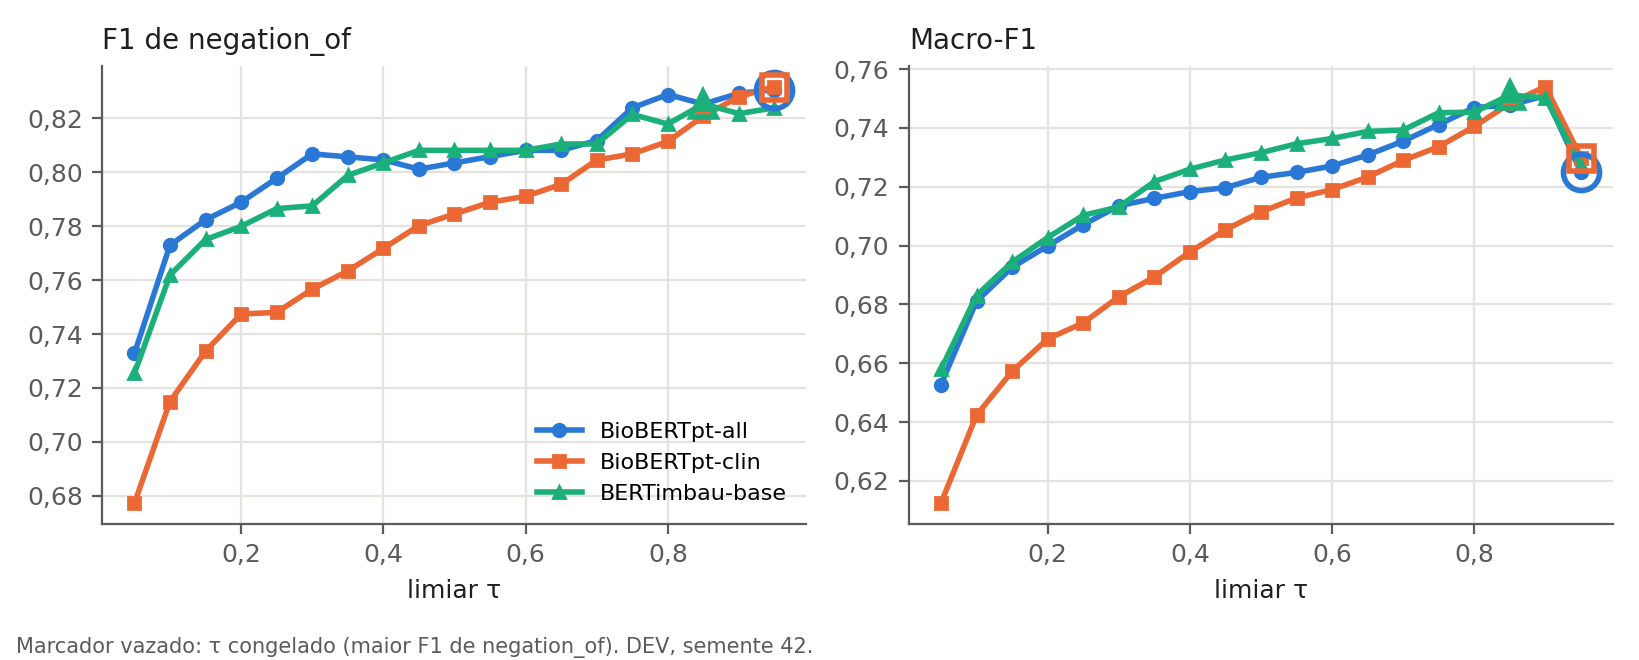
\includegraphics[width=\textwidth]{resultados/tau_two_stage_encoders.png}\\[4pt]
  {\footnotesize Fonte: elaborado pelo autor.}
\end{figure}

A Tabela~\ref{tab:two_stage_diag} mostra o que o estágio 1 encaminha com o limiar
congelado. Ele recupera de $88{,}7\%$ a $92{,}7\%$ dos pares \texttt{negation\_of},
mas só de $38{,}9\%$ a $68{,}3\%$ do conjunto de pares com relação, e, entre os pares
roteados que têm relação, o estágio 2 acerta o tipo em mais de $98\%$ dos casos nos
três \emph{encoders}. Nestas execuções, portanto, as perdas do Two-Stage
concentram-se no estágio 1 e no limiar, e não na distinção entre os tipos.

%% GERADO por analise/gerar_tabelas_etapa3.py -- nao edite a mao.
\begin{table}[htbp]
  \centering
  \caption{Two-Stage no DEV, por \emph{encoder}: o que o estágio 1 encaminha com o $\tau$ congelado e quanto o estágio 2 acerta do tipo.}
  \label{tab:two_stage_diag}
  \small\setlength{\tabcolsep}{4pt}
\adjustbox{max width=\textwidth}{%
  \begin{tabular}{lrrrrrr}
  \toprule
  \emph{Encoder} & $\tau$ & Roteados & \begin{tabular}[b]{@{}c@{}}Sem relação\\anotada\end{tabular} & \begin{tabular}[b]{@{}c@{}}\emph{Recall} est.\,1\\(neg)\end{tabular} & \begin{tabular}[b]{@{}c@{}}\emph{Recall} est.\,1\\(relação)\end{tabular} & \begin{tabular}[b]{@{}c@{}}Acerto\\do tipo\end{tabular} \\
  \midrule
BioBERTpt-all & 0{,}95 & 592 & 237 & 88{,}7\% & 38{,}9\% & 98{,}0\% \\
BioBERTpt-clin & 0{,}95 & 676 & 294 & 90{,}7\% & 41{,}8\% & 98{,}4\% \\
BERTimbau-base & 0{,}85 & 1\,494 & 870 & 92{,}7\% & 68{,}3\% & 98{,}6\% \\
  \bottomrule
  \end{tabular}}\\[2pt]
  {\footnotesize Diagnóstico do fluxo real, gravado na composição (\texttt{metricas.json}); não é resultado da arquitetura. Acerto do tipo: entre os pares roteados que têm relação anotada.}\\[4pt]
  {\footnotesize Fonte: elaborado pelo autor.}
\end{table}


A Tabela~\ref{tab:dev_comparacoes_ts} aplica ao DEV as comparações que o protocolo
prevê para o teste, estendidas aos três \emph{encoders}. No F1 de
\texttt{negation\_of}, o Two-Stage fica à frente do baseline do mesmo
\emph{encoder} ($+0{,}018$ a $+0{,}028$) e do baseline calibrado ($+0{,}021$), mas
nenhuma dessas diferenças é distinguível de zero. Em \texttt{associated\_with}, o
Two-Stage tem F1 menor que o do baseline com os dois BioBERTpt e que o do baseline
calibrado, com diferença detectada só por candidato, e maior com o BERTimbau-base,
com diferença detectada nos dois níveis. O baseline calibrado e o baseline diferem em
apenas $12$ pares; a diferença de $-0{,}0005$ em \texttt{associated\_with} entre eles
é detectada nos dois níveis, mas corresponde a esses poucos pares.

%% GERADO por analise/gerar_tabelas_etapa3.py -- nao edite a mao.
\begin{table}[htbp]
  \centering
  \caption{Comparações pareadas descritivas do Two-Stage e do baseline calibrado, no DEV, por métrica (as comparações que o protocolo prevê para o teste, aqui aplicadas ao DEV e estendidas aos três \emph{encoders}).}
  \label{tab:dev_comparacoes_ts}
  \small\renewcommand{\arraystretch}{1.2}\setlength{\tabcolsep}{3.5pt}
  \begin{tabular*}{\textwidth}{@{\extracolsep{\fill}}>{\raggedright\arraybackslash}p{3.85cm}lrcc}
  \toprule
  Comparação (A $-$ B) & \emph{Encoder} & $\Delta$ & IC95\% (candidato) & IC95\% (documento) \\
  \midrule
\multicolumn{5}{l}{\textit{Métrica:} F1 de \texttt{negation\_of}} \\
Two-Stage $-$ Baseline & BioBERTpt-all & $+0{,}0284$ & $[-0{,}008;\,+0{,}065]$ & $[-0{,}013;\,+0{,}074]$ \\
Two-Stage $-$ Baseline & BioBERTpt-clin & $+0{,}0179$ & $[-0{,}014;\,+0{,}049]$ & $[-0{,}018;\,+0{,}057]$ \\
Two-Stage $-$ Baseline & BERTimbau-base & $+0{,}0253$ & $[-0{,}005;\,+0{,}056]$ & $[-0{,}010;\,+0{,}065]$ \\
Two-Stage $-$ Baseline calibrado & BioBERTpt-all & $+0{,}0213$ & $[-0{,}011;\,+0{,}054]$ & $[-0{,}011;\,+0{,}056]$ \\
Baseline calibrado $-$ Baseline & BioBERTpt-all & $+0{,}0071$ & $[-0{,}012;\,+0{,}026]$ & $[-0{,}014;\,+0{,}030]$ \\
\midrule
\multicolumn{5}{l}{\textit{Métrica:} F1 de \texttt{associated\_with}} \\
Two-Stage $-$ Baseline & BioBERTpt-all & $-0{,}0421$ & $[-0{,}078;\,-0{,}006]$$^{\ast}$ & $[-0{,}107;\,+0{,}021]$ \\
Two-Stage $-$ Baseline & BioBERTpt-clin & $-0{,}0452$ & $[-0{,}079;\,-0{,}011]$$^{\ast}$ & $[-0{,}102;\,+0{,}009]$ \\
Two-Stage $-$ Baseline & BERTimbau-base & $+0{,}0434$ & $[+0{,}025;\,+0{,}061]$$^{\ast}$ & $[+0{,}013;\,+0{,}071]$$^{\ast}$ \\
Two-Stage $-$ Baseline calibrado & BioBERTpt-all & $-0{,}0416$ & $[-0{,}078;\,-0{,}005]$$^{\ast}$ & $[-0{,}107;\,+0{,}021]$ \\
Baseline calibrado $-$ Baseline & BioBERTpt-all & $-0{,}0005$ & $[-0{,}001;\,-0{,}0001]$$^{\ast}$ & $[-0{,}001;\,-0{,}0001]$$^{\ast}$ \\
\midrule
\multicolumn{5}{l}{\textit{Métrica:} Macro-F1} \\
Two-Stage $-$ Baseline & BioBERTpt-all & $+0{,}0062$ & $[-0{,}012;\,+0{,}024]$ & $[-0{,}021;\,+0{,}034]$ \\
Two-Stage $-$ Baseline & BioBERTpt-clin & $-0{,}0008$ & $[-0{,}017;\,+0{,}015]$ & $[-0{,}025;\,+0{,}023]$ \\
Two-Stage $-$ Baseline & BERTimbau-base & $+0{,}0285$ & $[+0{,}016;\,+0{,}041]$$^{\ast}$ & $[+0{,}012;\,+0{,}046]$$^{\ast}$ \\
Two-Stage $-$ Baseline calibrado & BioBERTpt-all & $+0{,}0040$ & $[-0{,}013;\,+0{,}021]$ & $[-0{,}021;\,+0{,}029]$ \\
Baseline calibrado $-$ Baseline & BioBERTpt-all & $+0{,}0023$ & $[-0{,}004;\,+0{,}009]$ & $[-0{,}005;\,+0{,}010]$ \\
  \bottomrule
  \end{tabular*}\\[2pt]
  \parbox{\textwidth}{\footnotesize Descritivas, no DEV: as épocas, $\tau$ e $t$ foram escolhidos neste mesmo conjunto; não substituem as comparações pré-registradas no teste. A e B usam o mesmo \emph{encoder}. $\Delta$: diferença observada A $-$ B no DEV completo. IC95\% (candidato): \emph{bootstrap} pareado que reamostra com reposição os 19\,064 pares candidatos, o do protocolo (10.000 reamostras, semente 42). IC95\% (documento): \emph{bootstrap} pareado que reamostra com reposição os 98 documentos do DEV que têm pares candidatos, cada um com todos os seus pares (10.000 reamostras, semente 42). As três métricas são calculadas sobre as mesmas reamostras de cada nível. Intervalos: percentis 2,5 e 97,5 das diferenças reamostradas. $^{\ast}$: intervalo que exclui o zero. Limites que arredondariam a zero com três casas aparecem com mais casas. O teste de McNemar dessas comparações está no Quadro~\ref{quad:mcnemar}.}\\[4pt]
  {\footnotesize Fonte: elaborado pelo autor.}
\end{table}


\section{Resultado exploratório}
\label{sec:resultados_exploratorios}

A variante Pair-Aware MLP, fora do protocolo, foi treinada com a mesma entrada, os
mesmos dados e a mesma seleção da Pair-Aware linear, mudando apenas a cabeça, e só com
o BioBERTpt-all. Ela teve \emph{recall} de \texttt{negation\_of} um pouco maior
($0{,}953$) e precisão menor ($0{,}715$), e terminou com F1 de $0{,}817$ e macro-F1 de
$0{,}737$, ambos abaixo da Pair-Aware linear, sem diferença detectada em nenhuma
métrica (Tabela~\ref{tab:dev_comparacoes_pa}). Por ser exploratório, esse resultado
não é evidência confirmatória.
